% latex2word README banner (24 cm x 8 cm, 3:1).
%
% Build (TeX Live or MiKTeX; the PGF dvisvgm driver writes SVG directly, no Ghostscript needed):
%   latex -interaction=nonstopmode -halt-on-error latex2word-banner.tex
%   dvisvgm --no-fonts --exact-bbox --precision=3 --output=latex2word-banner.svg latex2word-banner.dvi
%
% Everything is drawn here: no external images, logos or fonts beyond the TeX distribution.
\documentclass[dvisvgm,border=0pt]{standalone}
\usepackage[T1]{fontenc}
\usepackage{lmodern}% scalable math and typewriter fonts
\usepackage[scaled=0.95]{helvet}
\renewcommand{\familydefault}{\sfdefault}
\renewcommand{\ttdefault}{lmtt}
\usepackage{amsmath}
\usepackage{xcolor}
\usepackage{tikz}
\usetikzlibrary{arrows.meta,calc,positioning}

% ---------------------------------------------------------------- palette
\definecolor{bgA}{HTML}{0A1020}      % navy (left)
\definecolor{bgB}{HTML}{121633}      % navy with a violet cast (right)
\definecolor{panel}{HTML}{0F172A}    % editor background
\definecolor{panelHead}{HTML}{1A2338}
\definecolor{edge}{HTML}{2A3A5C}
\definecolor{ink}{HTML}{E2E8F0}      % light text
\definecolor{muted}{HTML}{8EA0BD}
\definecolor{dim}{HTML}{4B5B78}
\definecolor{cyan}{HTML}{22D3EE}
\definecolor{blue}{HTML}{3B82F6}
\definecolor{violet}{HTML}{A78BFA}
\definecolor{page}{HTML}{FFFFFF}
\definecolor{pageInk}{HTML}{1E293B}
\definecolor{pageMuted}{HTML}{64748B}
\definecolor{pageRule}{HTML}{CBD5E1}
\definecolor{heading}{HTML}{1D4ED8}

% ---------------------------------------------------------------- code helpers
\newcommand{\cmd}[1]{\textcolor{cyan}{\textbackslash #1}}
\newcommand{\grp}[1]{\textcolor{muted}{\{}\textcolor{violet}{#1}\textcolor{muted}{\}}}
\newcommand{\codefont}{\fontsize{8.6}{10}\selectfont\ttfamily}

\begin{document}
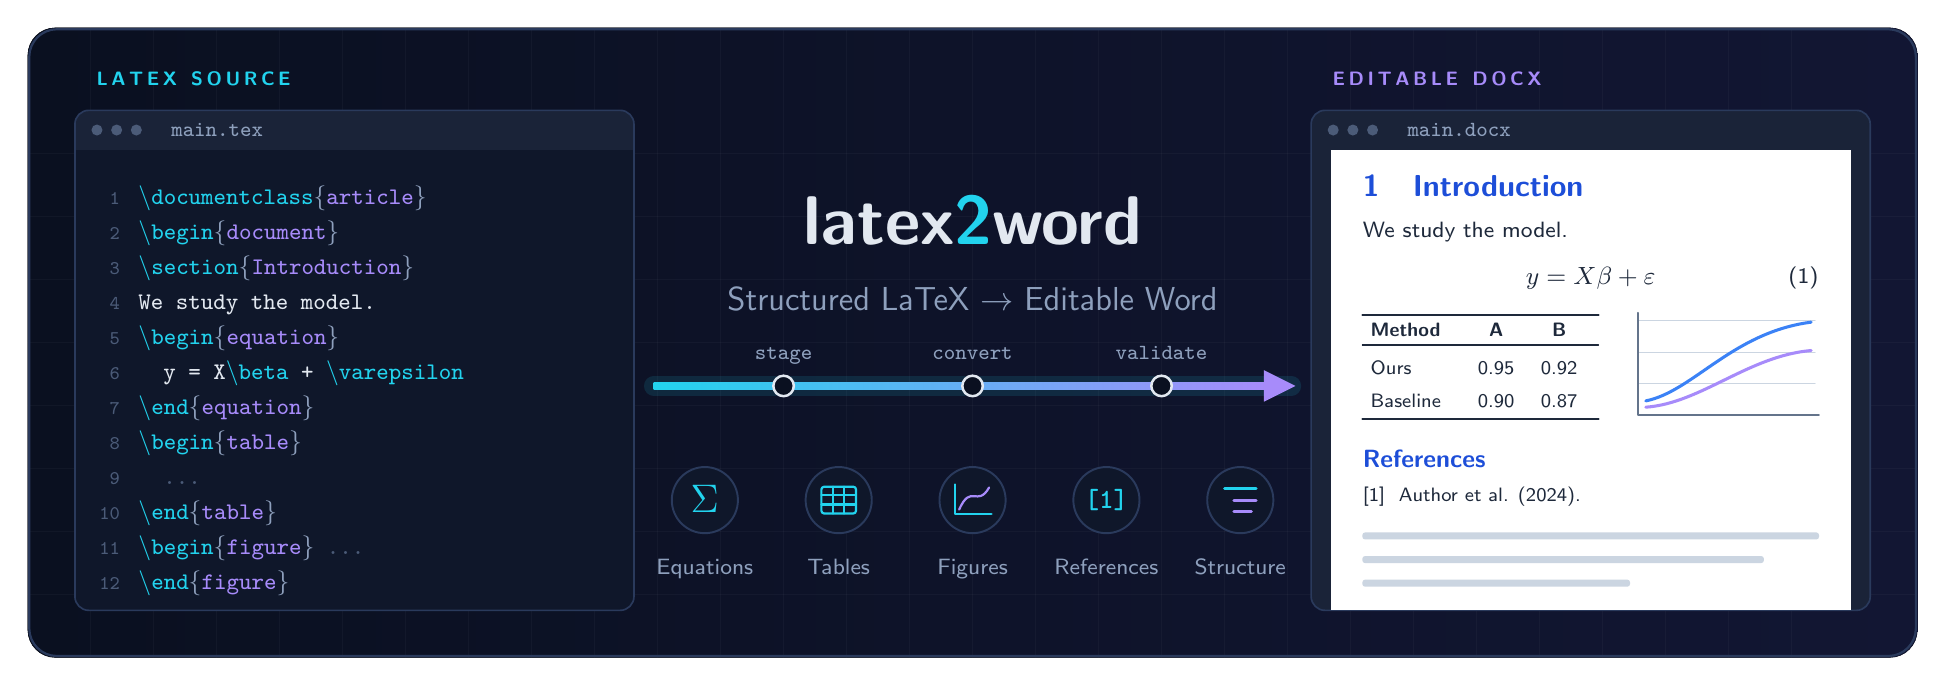
\begin{tikzpicture}[x=1cm,y=1cm,line cap=round,line join=round]
  % ---------------------------------------------------------------- background
  \useasboundingbox (0,0) rectangle (24,8);
  \fill[left color=bgA,right color=bgB,rounded corners=10pt] (0,0) rectangle (24,8);
  \begin{scope}
    \clip[rounded corners=10pt] (0,0) rectangle (24,8);
    \foreach \x in {0.8,1.6,...,23.2} \draw[ink,opacity=0.035,line width=0.4pt] (\x,0) -- (\x,8);
    \foreach \y in {0.8,1.6,...,7.2} \draw[ink,opacity=0.035,line width=0.4pt] (0,\y) -- (24,\y);
  \end{scope}
  \draw[edge,line width=0.8pt,rounded corners=10pt] (0.02,0.02) rectangle (23.98,7.98);% edge on dark themes

  % ---------------------------------------------------------------- left: LaTeX source
  \node[anchor=west,text=cyan,font=\fontsize{7.5}{9}\selectfont\bfseries] at (0.75,7.35) {L\,A\,T\,E\,X\ \ S\,O\,U\,R\,C\,E};
  \fill[panel,rounded corners=5pt] (0.6,0.6) rectangle (7.7,6.95);
  \fill[panelHead,rounded corners=5pt] (0.6,6.45) rectangle (7.7,6.95);
  \fill[panelHead] (0.6,6.45) rectangle (7.7,6.6);
  \draw[edge,rounded corners=5pt,line width=0.6pt] (0.6,0.6) rectangle (7.7,6.95);
  \foreach \c/\x in {dim/0.88,dim/1.13,dim/1.38} \fill[\c] (\x,6.7) circle (0.07);
  \node[anchor=west,text=muted,font=\fontsize{7.8}{9}\selectfont\ttfamily] at (1.7,6.7) {main.tex};
  \begin{scope}[every node/.style={anchor=base west,inner sep=0pt}]
    \foreach \n [count=\i] in {1,...,12} {
      \node[text=dim,font=\fontsize{7}{8}\selectfont\ttfamily,anchor=base east] at (1.18,6.2-0.445*\i) {\n};
    }
    \def\L#1#2{\node[text=ink,font=\codefont] at (1.4,6.2-0.445*#1) {#2};}
    \L{1}{\cmd{documentclass}\grp{article}}
    \L{2}{\cmd{begin}\grp{document}}
    \L{3}{\cmd{section}\grp{Introduction}}
    \L{4}{We study the model.}
    \L{5}{\cmd{begin}\grp{equation}}
    \L{6}{\ \ y = X\textcolor{cyan}{\textbackslash beta} + \textcolor{cyan}{\textbackslash varepsilon}}
    \L{7}{\cmd{end}\grp{equation}}
    \L{8}{\cmd{begin}\grp{table}}
    \L{9}{\ \ \textcolor{dim}{...}}
    \L{10}{\cmd{end}\grp{table}}
    \L{11}{\cmd{begin}\grp{figure}\ \textcolor{dim}{...}}
    \L{12}{\cmd{end}\grp{figure}}
  \end{scope}

  % ---------------------------------------------------------------- centre: title and pipeline
  \node[text=ink,font=\fontsize{40}{44}\selectfont\bfseries] at (12,5.55) {latex\textcolor{cyan}{2}word};
  \node[text=muted,font=\fontsize{12.5}{15}\selectfont] at (12,4.55) {Structured LaTeX $\rightarrow$ Editable Word};

  % pipeline arrow (soft glow underneath)
  \draw[cyan,opacity=0.12,line width=7pt] (7.95,3.45) -- (16.05,3.45);
  \shade[left color=cyan,right color=violet] (7.95,3.41) rectangle (15.75,3.49);
  \fill[violet] (15.7,3.25) -- (16.1,3.45) -- (15.7,3.65) -- cycle;
  \foreach \x/\stage in {9.6/stage,12/convert,14.4/validate} {
    \fill[bgA] (\x,3.45) circle (0.13);
    \draw[ink,line width=0.9pt] (\x,3.45) circle (0.13);
    \node[anchor=base,text=muted,font=\fontsize{7.8}{9}\selectfont\ttfamily] at (\x,3.78) {\stage};
  }

  % feature chips
  \tikzset{chip/.style={draw=edge,fill=panel,line width=0.7pt}}
  \def\chiplabel#1#2{\node[anchor=base,text=muted,font=\fontsize{7.6}{9}\selectfont] at (#1,1.05) {#2};}
  % Equations
  \fill[chip] (8.6,2.0) circle (0.42);
  \node[text=cyan,font=\fontsize{15}{15}\selectfont] at (8.6,2.02) {$\Sigma$};
  \chiplabel{8.6}{Equations}
  % Tables
  \fill[chip] (10.3,2.0) circle (0.42);
  \begin{scope}[shift={(10.3,2.0)},cyan,line width=0.8pt]
    \draw[rounded corners=1pt] (-0.22,-0.17) rectangle (0.22,0.17);
    \draw (-0.22,0.06) -- (0.22,0.06); \draw (-0.22,-0.055) -- (0.22,-0.055);
    \draw (-0.07,-0.17) -- (-0.07,0.17); \draw (0.07,-0.17) -- (0.07,0.17);
  \end{scope}
  \chiplabel{10.3}{Tables}
  % Figures
  \fill[chip] (12,2.0) circle (0.42);
  \begin{scope}[shift={(12,2.0)},line width=0.8pt]
    \draw[cyan] (-0.22,0.2) -- (-0.22,-0.18) -- (0.24,-0.18);
    \draw[violet] (-0.17,-0.12) .. controls (-0.02,0.22) and (0.06,-0.1) .. (0.21,0.16);
  \end{scope}
  \chiplabel{12}{Figures}
  % References
  \fill[chip] (13.7,2.0) circle (0.42);
  \node[text=cyan,font=\fontsize{10}{10}\selectfont\bfseries\ttfamily] at (13.7,2.0) {[1]};
  \chiplabel{13.7}{References}
  % Structure
  \fill[chip] (15.4,2.0) circle (0.42);
  \begin{scope}[shift={(15.4,2.0)},line width=1.1pt]
    \draw[cyan] (-0.2,0.15) -- (0.2,0.15);
    \draw[violet] (-0.08,0.0) -- (0.2,0.0);
    \draw[violet] (-0.08,-0.15) -- (0.14,-0.15);
  \end{scope}
  \chiplabel{15.4}{Structure}

  % ---------------------------------------------------------------- right: editable DOCX
  \node[anchor=west,text=violet,font=\fontsize{7.5}{9}\selectfont\bfseries] at (16.45,7.35) {E\,D\,I\,T\,A\,B\,L\,E\ \ D\,O\,C\,X};
  \fill[panelHead,rounded corners=5pt] (16.3,0.6) rectangle (23.4,6.95);
  \draw[edge,rounded corners=5pt,line width=0.6pt] (16.3,0.6) rectangle (23.4,6.95);
  \foreach \x in {16.58,16.83,17.08} \fill[dim] (\x,6.7) circle (0.07);
  \node[anchor=west,text=muted,font=\fontsize{7.8}{9}\selectfont\ttfamily] at (17.4,6.7) {main.docx};
  % page
  \fill[page] (16.55,0.6) rectangle (23.15,6.45);
  \begin{scope}[every node/.style={inner sep=0pt}]
    \node[anchor=base west,text=heading,font=\fontsize{10.5}{12}\selectfont\bfseries] at (16.95,5.85) {1\quad Introduction};
    \node[anchor=base west,text=pageInk,font=\fontsize{8}{10}\selectfont] at (16.95,5.33) {We study the model.};
    \node[text=pageInk,font=\fontsize{9.5}{11}\selectfont] at (19.85,4.82) {$y = X\beta + \varepsilon$};
    \node[anchor=east,text=pageInk,font=\fontsize{8}{10}\selectfont] at (22.75,4.82) {(1)};
    % table
    \draw[pageInk,line width=0.7pt] (16.95,4.35) -- (19.95,4.35);
    \draw[pageInk,line width=0.4pt] (16.95,3.97) -- (19.95,3.97);
    \draw[pageInk,line width=0.7pt] (16.95,3.03) -- (19.95,3.03);
    \foreach \y/\a/\b/\c/\w in {4.08/Method/A/B/\bfseries,3.6/Ours/0.95/0.92/,3.18/Baseline/0.90/0.87/} {
      \node[anchor=base west,text=pageInk,font=\fontsize{7.4}{9}\selectfont\w] at (17.05,\y) {\a};
      \node[anchor=base,text=pageInk,font=\fontsize{7.4}{9}\selectfont\w] at (18.65,\y) {\b};
      \node[anchor=base,text=pageInk,font=\fontsize{7.4}{9}\selectfont\w] at (19.45,\y) {\c};
    }
    % plot
    \begin{scope}[shift={(20.45,3.08)}]
      \draw[pageRule,line width=0.4pt] (0,0.4) -- (2.25,0.4) (0,0.8) -- (2.25,0.8) (0,1.2) -- (2.25,1.2);
      \draw[pageMuted,line width=0.6pt] (0,1.3) -- (0,0) -- (2.3,0);
      \draw[blue,line width=1.1pt] (0.1,0.18) .. controls (0.7,0.3) and (1.2,1.05) .. (2.2,1.18);
      \draw[violet,line width=1.1pt] (0.1,0.1) .. controls (0.8,0.15) and (1.4,0.75) .. (2.2,0.82);
    \end{scope}
    % references
    \node[anchor=base west,text=heading,font=\fontsize{8.6}{10}\selectfont\bfseries] at (16.95,2.42) {References};
    \node[anchor=base west,text=pageInk,font=\fontsize{7.4}{9}\selectfont] at (16.95,1.98) {[1]\ \ Author et al. (2024).};
    % more text, suggested
    \foreach \y/\w in {1.5/5.8,1.2/5.1,0.9/3.4} \fill[pageRule,rounded corners=1pt] (16.95,\y) rectangle (16.95+\w,\y+0.09);
  \end{scope}
\end{tikzpicture}
\end{document}
